% ============================================================
%  Invoy VLM – 15-minute Beamer presentation
%  Audience: technical / academic
% ============================================================
\documentclass[10pt, aspectratio=169]{beamer}

% ---------- Theme & colour ----------------------------------------
\usetheme{Madrid}
\definecolor{invoyblue}{RGB}{31,119,180}   % #1f77b4 – matches figure palette
\usecolortheme[named=invoyblue]{structure}

% Model highlight colours
\definecolor{col2b}{RGB}{31,119,180}    % blue  – 2B
\definecolor{col3b}{RGB}{255,127,14}    % orange – 3B
\definecolor{col7b}{RGB}{44,160,44}     % green  – 7B

% ---------- Packages ----------------------------------------------
\usepackage[T1]{fontenc}
\usepackage{lmodern}
\usepackage{graphicx}
\graphicspath{{figures/}}
\usepackage{booktabs}
\usepackage{xcolor}
\usepackage{amsmath}

% ---------- Footer / nav ------------------------------------------
\setbeamertemplate{navigation symbols}{}
\setbeamertemplate{footline}[frame number]

% ---------- Metadata ----------------------------------------------
\title[Invoy VLM]{Invoy VLM: Benchmarking Local Vision-Language Models\\
       for Continuous Desktop Activity Tracking}
\author{Hamza}
\date{April 2026}
\institute{\texttt{invoy\_sdk} Research Project}

% ==================================================================
\begin{document}

% ------------------------------------------------------------------
% SLIDE 1 – Title
% ------------------------------------------------------------------
\begin{frame}
  \titlepage
\end{frame}

% ------------------------------------------------------------------
% SECTION 1 – Introduction
% ------------------------------------------------------------------
\section{Introduction}

% SLIDE 2 – Motivation
\begin{frame}{Motivation}
  \begin{columns}[T]
    \begin{column}{0.48\textwidth}
      \textbf{The problem}
      \begin{itemize}
        \item Desktop activity tracking = knowing what a user is working on
        \item App-level hooks cover only instrumented apps — no unified view
        \item Manual logging: tedious and inaccurate
      \end{itemize}
    \end{column}
    \begin{column}{0.48\textwidth}
      \textbf{The VLM opportunity}
      \begin{itemize}
        \item Periodic screenshot $\to$ local VLM $\to$ natural-language activity log
        \item Universal, application-agnostic
        \item Privacy-preserving — no data leaves the machine
        \item \textbf{Open question:} do compact 2–7B models actually work?
      \end{itemize}
    \end{column}
  \end{columns}
\end{frame}

% SLIDE 3 – Research Questions
\begin{frame}{Research Questions}
  \begin{block}{RQ1 — Quality vs.\ parameter count}
    How does activity description quality scale from 2B to 7B parameters?
  \end{block}
  \vspace{0.4em}
  \begin{block}{RQ2 — Architecture vs.\ parameters}
    Does the newer Qwen2.5-VL architecture outperform Qwen2-VL at comparable size (3B)?
  \end{block}
  \vspace{0.4em}
  \begin{block}{RQ3 — Change detection}
    Can any compact model reliably detect task switches from periodic screenshots?
  \end{block}
\end{frame}

% ------------------------------------------------------------------
% SECTION 2 – System & Data
% ------------------------------------------------------------------
\section{System \& Data}

% SLIDE 4 – The Invoy System
\begin{frame}{The Invoy System}
  \begin{columns}[T]
    \begin{column}{0.55\textwidth}
      \textbf{Pipeline}
      \medskip

      \begin{tabular}{ccc}
        \fbox{Screenshot (10 s)} & $\!\!\to\!\!$ & \fbox{VLM inference} \\[4pt]
        & & $\downarrow$ \\[2pt]
        & & \fbox{SQLite log}
      \end{tabular}

      \bigskip
      \textbf{Two prompts per frame:}
      \begin{itemize}
        \item \textbf{Activity prompt} — current screenshot $\to$ 2–3 sentence description
        \item \textbf{Change prompt} — prev text + curr text (\emph{text only}) $\to$ what changed?
      \end{itemize}
    \end{column}
    \begin{column}{0.42\textwidth}
      \begin{block}{Design rationale}
        \begin{itemize}
          \item Image comparison would double inference cost at 10-s cadence
          \item Text-only change prompt keeps pipeline within resource budget
          \item Runs fully offline on consumer hardware
        \end{itemize}
      \end{block}
    \end{column}
  \end{columns}
\end{frame}

% SLIDE 5 – Models & Dataset
\begin{frame}{Models \& Dataset}
  \begin{columns}[T]
    \begin{column}{0.52\textwidth}
      \textbf{Models evaluated}
      \medskip

      \begin{tabular}{llll}
        \toprule
        Label & Family & Params & VRAM \\
        \midrule
        \textcolor{col2b}{\textbf{2B}} & Qwen2-VL   & $\sim$2B & $\sim$5 GB \\
        \textcolor{col3b}{\textbf{3B}} & Qwen2.5-VL & $\sim$3B & $\sim$7 GB \\
        \textcolor{col7b}{\textbf{7B}} & Qwen2-VL   & $\sim$7B & $\sim$14 GB \\
        \bottomrule
      \end{tabular}

      \vspace{0.4em}
      {\small 7B used as pseudo ground-truth reference}
    \end{column}
    \begin{column}{0.45\textwidth}
      \textbf{Dataset}
      \begin{itemize}
        \item \textbf{136 frames} over 22.8 minutes
        \item Real Linux workstation session (16 Mar 2026)
        \item Activities: Python development in VS Code, terminal work, web browsing (incl.\ grade portal)
        \item 16 manually annotated task-switch transitions
      \end{itemize}
    \end{column}
  \end{columns}
\end{frame}

% ------------------------------------------------------------------
% SECTION 3 – Evaluation
% ------------------------------------------------------------------
\section{Evaluation}

% SLIDE 6 – Evaluation Methodology
\begin{frame}{Evaluation Methodology}
  \begin{columns}[T]
    \begin{column}{0.24\textwidth}
      \begin{block}{Activity quality}
        \begin{itemize}\small
          \item Token length
          \item Specificity score
          \item Hedging rate
        \end{itemize}
      \end{block}
    \end{column}
    \begin{column}{0.24\textwidth}
      \begin{block}{Change-Delta F1}
        \begin{itemize}\small
          \item F1 between change-text tokens and symmetric difference of consecutive activity texts
          \item Precision penalises hallucination
          \item Recall rewards coverage
        \end{itemize}
      \end{block}
    \end{column}
    \begin{column}{0.24\textwidth}
      \begin{block}{Change detection}
        \begin{itemize}\small
          \item Precision / Recall / F1
          \item vs.\ 16 keyword-transition ground-truth events
        \end{itemize}
      \end{block}
    \end{column}
    \begin{column}{0.24\textwidth}
      \begin{block}{Cross-model agreement}
        \begin{itemize}\small
          \item TF-IDF cosine similarity
          \item ROUGE-L
          \item Jaccard
          \item vs.\ 7B reference
        \end{itemize}
      \end{block}
    \end{column}
  \end{columns}

  \vspace{0.8em}
  \small
  \textbf{Change-Delta F1 formal definition:}
  \[
    \delta = \mathrm{tok}(a_{t-1}) \mathbin{\triangle} \mathrm{tok}(a_t),\quad
    \mathrm{CDF1} = \frac{2\,|\delta \cap \mathrm{tok}(c_t)|}{|\delta| + |\mathrm{tok}(c_t)|}
  \]
  where $a_t$ = activity text, $c_t$ = change text at frame $t$.
\end{frame}

% ------------------------------------------------------------------
% SECTION 4 – Results
% ------------------------------------------------------------------
\section{Results}

% SLIDE 7 – Activity Description Quality
\begin{frame}{Activity Description Quality (RQ1)}
  \begin{center}
    \includegraphics[width=0.85\textwidth]{01_quality_metrics_bar}
  \end{center}
  \vspace{-0.5em}
  \begin{columns}[T]
    \begin{column}{0.6\textwidth}
      \begin{itemize}
        \item \textcolor{col7b}{\textbf{7B}} richest: 44.7 tokens, lowest hedging (0.006)
        \item \textcolor{col2b}{\textbf{2B}} counter-intuitive: \emph{highest} specificity (0.038 $>$ 7B's 0.033)
        \item \textcolor{col3b}{\textbf{3B}} most concise: 25.9 tokens, specificity 0.016
      \end{itemize}
    \end{column}
    \begin{column}{0.38\textwidth}
      \begin{alertblock}{Finding}
        Parameter count drives richness; 2B's keyword-anchoring style produces the highest concrete identifier density.
      \end{alertblock}
    \end{column}
  \end{columns}
\end{frame}

% SLIDE 8 – Architecture vs Parameters (RQ2)
\begin{frame}{Architecture vs.\ Parameters (RQ2)}
  \begin{columns}[T]
    \begin{column}{0.48\textwidth}
      \begin{center}
        \includegraphics[width=\textwidth]{08_radar_overall}
      \end{center}
    \end{column}
    \begin{column}{0.48\textwidth}
      \vspace{1em}
      \begin{itemize}
        \item \textcolor{col3b}{\textbf{3B}} polygon is \textbf{interior to both 2B and 7B on every activity axis}
        \item Newer Qwen2.5-VL architecture does \emph{not} compensate for lower parameter count
        \item Likely: OCR / spatial improvements manifest at 7B+, not 3B
      \end{itemize}
      \vspace{0.8em}
      \begin{alertblock}{Bottom line}
        \textcolor{col3b}{\textbf{Avoid 3B.}} The extra VRAM over 2B yields no benefit.
      \end{alertblock}
    \end{column}
  \end{columns}
\end{frame}

% SLIDE 9 – Session Structure
\begin{frame}{Session Structure}
  \begin{center}
    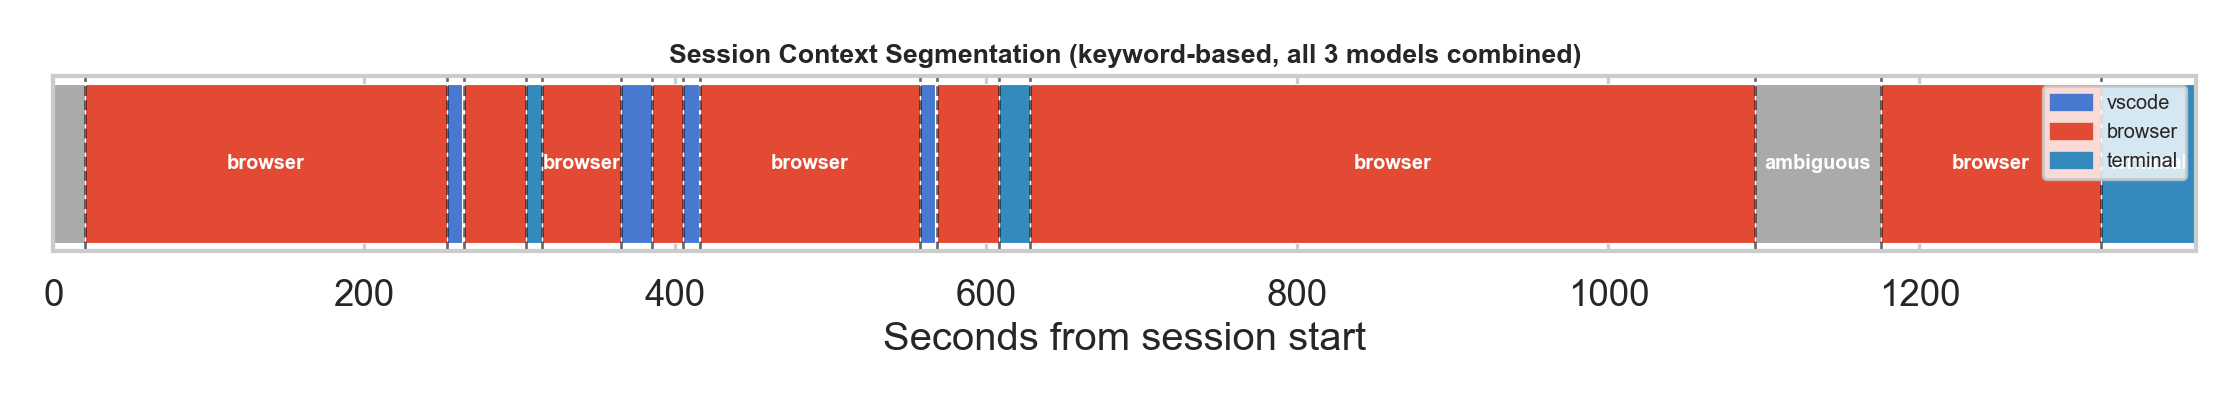
\includegraphics[width=0.9\textwidth]{s2_segment_timeline}
  \end{center}
  \vspace{-0.4em}
  \begin{columns}
    \begin{column}{0.5\textwidth}
      \begin{itemize}
        \item $\sim$80\% of frames are \textbf{browser} context
        \item VS Code: brief 1–2 frame bursts only
      \end{itemize}
    \end{column}
    \begin{column}{0.5\textwidth}
      \begin{itemize}
        \item Terminal: only in final 6 frames (131–136)
        \item Both task-switch anchors (frame $\sim$40, $\sim$110) recovered automatically
      \end{itemize}
    \end{column}
  \end{columns}
\end{frame}

% SLIDE 10 – Context-Dependent Agreement
\begin{frame}{Context-Dependent Agreement}
  \begin{center}
    \includegraphics[width=0.9\textwidth]{s3_segment_agreement}
  \end{center}
  \vspace{-0.4em}
  \begin{itemize}
    \item Longest stable browser segments (fr 63–108 and 117–130): \textcolor{col2b}{\textbf{2B cosine 0.40}} vs \textcolor{col3b}{3B 0.33}
    \item In short/transitional segments: 3B occasionally wins on a per-segment basis
    \item \textbf{2B's overall advantage is concentrated in stable, content-rich portions of the session}
  \end{itemize}
\end{frame}

% SLIDE 11 – Change Detection (RQ3 part 1)
\begin{frame}{Change Detection: The Critical Finding (RQ3)}
  \begin{columns}[T]
    \begin{column}{0.52\textwidth}
      \begin{center}
        \includegraphics[width=\textwidth]{s4_change_detection_pr}
      \end{center}
    \end{column}
    \begin{column}{0.45\textwidth}
      \vspace{0.5em}
      \begin{center}
        \Large
        \textbf{Precision $\approx$ 0.12}\\[4pt]
        \textbf{Recall $\approx$ 1.0}\\[4pt]
        \textbf{F1 $\approx$ 0.21}
      \end{center}
      \vspace{0.6em}
      \begin{itemize}
        \item 16 real transitions in 136 frames
        \item Models fire change events on $\sim$130 frames — \textbf{indiscriminate}
        \item All three models behave identically — model size does not help
      \end{itemize}
      \vspace{0.4em}
      \begin{alertblock}{Key implication}
        A downstream classifier is \textbf{required} before change texts are usable.
      \end{alertblock}
    \end{column}
  \end{columns}
\end{frame}

% SLIDE 12 – Change-Delta F1 (RQ3 part 2)
\begin{frame}{Change-Delta F1: Grounding Quality (RQ3)}
  \begin{columns}[T]
    \begin{column}{0.52\textwidth}
      \begin{center}
        \includegraphics[width=\textwidth]{07_change_delta_f1_bar}
      \end{center}
    \end{column}
    \begin{column}{0.45\textwidth}
      \vspace{0.5em}
      \begin{center}
        \large
        \textcolor{col2b}{\textbf{2B: 0.334}}\quad
        \textcolor{col3b}{3B: 0.269}\quad
        \textcolor{col7b}{7B: 0.200}
      \end{center}
      \vspace{0.6em}
      \begin{itemize}
        \item \textbf{Reverse of activity quality ranking}
        \item 7B paraphrases semantically but is lexically ungrounded
        \item 2B echoes delta tokens directly $\to$ higher CDF1
        \item Spearman $r > 0.81$ for all models — all scale with drift magnitude
      \end{itemize}
      \vspace{0.4em}
      \begin{block}{Interpretation}
        CDF1 measures \emph{responsiveness}, not fluency.
      \end{block}
    \end{column}
  \end{columns}
\end{frame}

% SLIDE 13 – OLS Regression
\begin{frame}{OLS Regression: Same Intercept, Different Slope}
  \begin{center}
    \includegraphics[width=0.88\textwidth]{07b_drift_vs_cdf1_scatter}
  \end{center}
  \vspace{-0.5em}
  \begin{columns}
    \begin{column}{0.45\textwidth}
      \begin{tabular}{lcc}
        \toprule
        Model & Slope & Intercept \\
        \midrule
        \textcolor{col2b}{\textbf{2B}} & \textbf{0.697} & 0.015 \\
        \textcolor{col3b}{3B}          & 0.545          & 0.012 \\
        \textcolor{col7b}{7B}          & 0.394          & 0.017 \\
        \bottomrule
      \end{tabular}
    \end{column}
    \begin{column}{0.52\textwidth}
      \begin{alertblock}{Finding}
        2B's grounding rises \textbf{77\% faster} with activity drift than 7B's.
        Intercepts are near-identical ($\leq 0.017$) — the difference is
        \emph{responsiveness}, not baseline.
      \end{alertblock}
    \end{column}
  \end{columns}
\end{frame}

% ------------------------------------------------------------------
% SECTION 5 – Discussion & Next Steps
% ------------------------------------------------------------------
\section{Discussion \& Next Steps}

% SLIDE 14 – Deployment Guidance
\begin{frame}{Deployment Guidance}
  \begin{columns}[T]
    \begin{column}{0.32\textwidth}
      \begin{block}{\textcolor{col7b}{\textbf{Use 7B when\ldots}}}
        \begin{itemize}
          \item $\geq$14 GB VRAM available
          \item Downstream: embeddings or LLM pipeline
          \item Fluency and hedging calibration matter
        \end{itemize}
      \end{block}
    \end{column}
    \begin{column}{0.32\textwidth}
      \begin{block}{\textcolor{col2b}{\textbf{Use 2B when\ldots}}}
        \begin{itemize}
          \item $\sim$5 GB VRAM budget
          \item Downstream: keyword parsing
          \item Highest CDF1 (0.334) \& Spearman $r$ (0.863)
        \end{itemize}
      \end{block}
    \end{column}
    \begin{column}{0.32\textwidth}
      \begin{alertblock}{\textcolor{col3b}{\textbf{Avoid 3B}}}
        \begin{itemize}
          \item Inferior to 2B on \emph{every} measured dimension
          \item Extra VRAM cost yields no benefit
        \end{itemize}
      \end{alertblock}
    \end{column}
  \end{columns}
  \vspace{0.8em}
  \begin{center}
    \begin{beamercolorbox}[sep=4pt,center,rounded=true]{structure}
      \textbf{Warning:} Post-process ALL change texts — raw VLM output is not selective
      (precision 0.12, recall 1.0)
    \end{beamercolorbox}
  \end{center}
\end{frame}

% SLIDE 15 – Future Work
\begin{frame}{Future Work}
  \begin{columns}[T]
    \begin{column}{0.48\textwidth}
      \begin{block}{1. Temporal Classifier}
        Lightweight binary model on consecutive activity text pairs.
        Use 7B descriptions as pseudo-labels to generate training data without manual annotation.
      \end{block}
      \vspace{0.4em}
      \begin{block}{2. Semantic CDF1}
        Replace token overlap with embedding cosine similarity.
        Credits 7B's paraphrasing style; gives a model-agnostic grounding score.
      \end{block}
    \end{column}
    \begin{column}{0.48\textwidth}
      \begin{block}{3. Constrained Prompts}
        Structured YES/NO task-switch question forces an explicit decision signal.
        Transforms change detection from post-hoc parsing to direct classification.
      \end{block}
      \vspace{0.4em}
      \begin{block}{4. Fine-tuning}
        200–300 human-annotated transition pairs for a specialised change-detection head.
        Target: precision $>$ 0.5 while maintaining recall $>$ 0.8.
      \end{block}
    \end{column}
  \end{columns}
\end{frame}

% SLIDE 16 – Conclusion
\begin{frame}{Conclusion}
  \begin{itemize}
    \setlength\itemsep{0.55em}
    \item \textbf{Parameter count} governs activity description quality — \textcolor{col7b}{7B} leads on richness, fluency, and confidence calibration
    \item \textbf{Newer architecture $\neq$ better} — Qwen2.5-VL \textcolor{col3b}{3B} is uniformly below Qwen2-VL \textcolor{col2b}{2B} on all activity metrics
    \item \textbf{Change texts are indiscriminate} — precision 0.12, recall 1.0; a classifier layer is \emph{mandatory} before deployment
    \item \textcolor{col2b}{\textbf{2B is the optimal compact model}} — highest CDF1 (0.334), steepest drift-responsiveness slope (0.697)
  \end{itemize}
  \vspace{1em}
  \begin{center}
    \textit{Invoy SDK, evaluation scripts, and databases are open.}
  \end{center}
  \vspace{0.4em}
  \begin{center}
    \large\textbf{Thank you}
  \end{center}
\end{frame}

\end{document}
